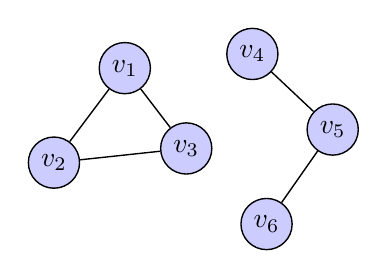
\begin{tikzpicture}[
  scale=0.6,
  vnode/.style={circle, fill=blue!20, draw=black, line width=0.5pt, inner sep=2pt, minimum size=6.5mm},
  edge/.style={line width=0.5pt, draw=black}
]

  % --- Componente 1 (Triángulo) ---
  \node[vnode] (v1) at (-2.5, 2.5) {$v_1$};
  \node[vnode] (v2) at (-4.0, 0.5) {$v_2$};
  \node[vnode] (v3) at (-1.2, 0.8) {$v_3$};

  \draw[edge] (v1) -- (v2) -- (v3) -- (v1);

  % --- Componente 2 (Camino/Trayectoria) ---
  \node[vnode] (v4) at (0.2, 2.8) {$v_4$};
  \node[vnode] (v5) at (1.9, 1.2) {$v_5$};
  \node[vnode] (v6) at (0.5, -0.8) {$v_6$};

  \draw[edge] (v4) -- (v5);
  \draw[edge] (v5) -- (v6);

\end{tikzpicture}
